% A skeleton file for producing Computer Engineering reports
% https://kgcoe-git.rit.edu/jgm6496/KGCOEReport_template

\documentclass[CMPE]{KGCOEReport}

% The following should be changed to represent your personal information
\newcommand{\classCode}{CMPE 160}  % 4 char code with number
\newcommand{\name}{Andrei Tumbar}
\newcommand{\LabSectionNum}{4}
\newcommand{\LabInstructor}{Mr.\ Byers}	% The slash is to tell LaTeX that the period is between words
												% not sentences so it spaces correctly. It won't appear in the
												% final pdf
\newcommand{\TAs}{Sam Myers \\ Kobe Balin \\ Georgi Thomas}
\newcommand{\LectureSectionNum}{1}
\newcommand{\LectureInstructor}{Mr.\ Cliver}
\newcommand{\exerciseNumber}{11}
\newcommand{\exerciseDescription}{Modeling of Combinational Circuits Using Concurrent and Sequential Statements}
\newcommand{\dateDone}{April 16th}
\newcommand{\dateSubmitted}{April 23rd}

\graphicspath{{./lab11_media/}}

\usepackage{circuitikz}
\usepackage{tikz}
\usepackage{multirow}
\usepackage{titlesec}
\usepackage{float}
\usepackage{pgfplots, pgfplotstable}
\usepackage{lmodern}
\usepackage{siunitx}
\usepackage{subcaption}

\usepackage[usestackEOL]{stackengine}
\usepackage{scalerel}

\usepackage{hhline}
\usepackage{kmap}
\usepackage[T1]{fontenc}
\usetikzlibrary{automata, positioning, arrows}
\usepackage{amsmath}

\def\lbar#1{\ThisStyle{%
  \setbox0=\hbox{$\SavedStyle#1$}%
  \stackengine{2.2\LMpt}{$\SavedStyle#1$}{\rule{\wd0}{0.1\LMpt}}{O}{c}{F}{F}{S}%
}}

\ctikzset{bipoles/not port/circle width=.4}
\ctikzset{tripoles/american xor port/height/.initial=.4}
\ctikzset{tripoles/american xor port/width/.initial=.6}

\DeclareFontFamily{U}{mathx}{\hyphenchar\font45}
\DeclareFontShape{U}{mathx}{m}{n}{ <-> mathx10 }{}
\DeclareSymbolFont{mathx}{U}{mathx}{m}{n}
\DeclareFontSubstitution{U}{mathx}{m}{n}
\DeclareMathAccent{\widebar}{\mathalpha}{mathx}{"73}

\makeatletter
\newcommand{\cwidebar}[2][0]{{\mathpalette\@cwidebar{{#1}{#2}}}}
\newcommand{\@cwidebar}[2]{\@cwideb@r{#1}#2}
\newcommand{\@cwideb@r}[3]{%
  \sbox\z@{$\m@th\mkern-#2mu#3\mkern#2mu$}%
  \widebar{\box\z@}%
}
\makeatother

\begin{document}
\maketitle

\section*{Abstract}

In this laboratory exercise a 4:1 multiplexor circuit was implemented in VHDL. Dataflow, behavioral, and structural implementations were performed. The 74LS153 chip was simulated in ModelSim with varying input sequences to varify integrity of functionallity. The exercise was successful in simulating the chip as the outputs of the mux had expected values and predicted propagation delays.

\section*{Design Methodology}

The circuit in question is meant to emulate the 74LS153 chip which includes two 4:1 multiplexors with active low enable on each. The select lines are the same for both multiplexors however each have a separate set of input lines.

\begin{figure}[h]
\centering
\begin{circuitikz}[american, PH/.append style={font=\scriptsize,inner ysep=2pt,inner xsep=5pt},
                   PV/.append style={PH,inner ysep=2pt,inner xsep=2pt}]
	\ctikzset{multipoles/thickness=4}
	\ctikzset{multipoles/external pins thickness=2}
	
	\node [label={[label distance=-.9cm,text depth=0em,rotate=-90]right:74LS153}] at (-0.13,0) {};
	
	\draw (0,0) node[dipchip,
		num pins=16,
		external pins width=0.3,
		external pad fraction=4](ls153){};
	
	\draw
		(ls153.pin 1) node [PH, left] {$\widebar{G_1}$}
		(ls153.pin 2) node [PH, left] {$B$}
		(ls153.pin 3) node [PH, left] {$1C_3$}
		(ls153.pin 4) node [PH, left] {$1C_2$}
		(ls153.pin 5) node [PH, left] {$1C_1$}
		(ls153.pin 6) node [PH, left] {$1C_0$}
		(ls153.pin 7) node [PH, left] {$1Y$}
		(ls153.pin 8) node [PH, left] {GND}
	;
	
	\draw 
		(ls153.pin 16) node [PH, right] {VCC}
		(ls153.pin 15) node [PH, right] {$\widebar{G_2}$}
		(ls153.pin 14) node [PH, right] {$A$}
		(ls153.pin 13) node [PH, right] {$2C_3$}
		(ls153.pin 12) node [PH, right] {$2C_2$}
		(ls153.pin 11) node [PH, right] {$2C_1$}
		(ls153.pin 10) node [PH, right] {$2C_0$}
		(ls153.pin 9)  node [PH, right] {$2Y$}
	;

\end{circuitikz}

\caption{74LS153 chip}
\label{fig:74ls153}
\end{figure}

Figure \ref{fig:74ls153} shows the pin configuration on the 74LS153. In the figure, $A$ and $B$ are the select lines, $\widebar{G_1}$ and $\widebar{G_2}$ are the enable pins and are labeled as such to indicate their active low behavior. The two four bit numbers $1C$ and $2C$ are the input pins for each multiplexor. Finally the outputs are labeled $1Y$ and $2Y$.\\

The VHDL program made to emulate the chip was implemented in three different ways: Dataflow, Behavioral, and Structural. Dataflow did not take into account the time constraints of the gates inside but rather only the functionality of it. Therefore changes in input would result in immediate change in output. Behavioral was implemented similarly to the dataflow, however, the worst case scenario propagation delay of $22\,\si{\nano\s}$ was taken into account.\\

Finally the structural was implemented using an entity for every gate and their own delays.
\pagebreak

\begin{table}[htbp]
\renewcommand{\arraystretch}{1.2}
\setlength{\tabcolsep}{12pt}
\begin{center}
\caption{Gate and their delays in the 74LS153}
\begin{tabular}{c|c|c}
Gate & Delay (ns) & Input\\\hline
OR & 7 & 4\\\hline
AND & 7 & 4\\\hline
NOT & 4 & 1 

\label{tab:gates}
\end{tabular}
\end{center}
\end{table}

Each gate was written separately and given their own delay. This final structural implementation provided a more realistic emulation of the propagation delay experienced on the actual chip.

\section*{Results and Analysis}

A test bench is required to test the VHDL circuit. To do this an input sequence must be chosen. The first input sequence started with a 4-bit number and performed a circular left-shift every $50\,\si{\nano\s}$. The select lines which created a 2-bit number (BA) was incremented every $100\,\si{\nano\s}$. The input consisted of two of these 4-bit numbers that would each shift left twice on every interval. To maximize the number of changes in input, these two 4-bit numbers swaped the input they were going to on every $100\,\si{\nano\s}$ cycle.

\begin{table}[htbp]
\renewcommand{\arraystretch}{1.2}
\begin{center}
\caption{Test set 1}
\begin{tabular}{|c|c|c|cccc|}
\hline
G & B & A & C3 & C2 & C1 & C0\\\hline
0 & 0 & 0 & 1 & 1 & 1 & 0\\\hline
0 & 0 & 0 & 0 & 0 & 0 & 1\\\hhline{|=|=|=|====|}
0 & 0 & 1 & 1 & 1 & 0 & 1\\\hline
0 & 0 & 1 & 0 & 0 & 1 & 0\\\hhline{|=|=|=|====|}
0 & 1 & 0 & 1 & 0 & 1 & 1\\\hline
0 & 1 & 0 & 0 & 1 & 0 & 0\\\hhline{|=|=|=|====|}
0 & 1 & 1 & 0 & 1 & 1 & 1\\\hline
0 & 1 & 1 & 1 & 0 & 0 & 0\\\hline
\end{tabular}
\label{tab:set1}
\end{center}
\end{table}

Table \ref{tab:set1} shows the inputs and the select line combinations. The double row splits indicate a passing of $100\,\si{\nano\s}$. The first row of each grouping shows the first 4-bit number being left shifted. The row each mux input will see changes on every select line change.\\

The second test set was meant to test every select combination of two different four bit numbers.
\pagebreak

\begin{table}[htbp]
\renewcommand{\arraystretch}{1.2}
\begin{center}
\caption{Test set 2}
\begin{tabular}{|c|c|c|cccc|}
\hline
G & B & A & C3 & C2 & C1 & C0\\\hline
0 & 0 & 0 & 1 & 0 & 1 & 0\\\hline
0 & 0 & 1 & 1 & 0 & 1 & 0\\\hline
0 & 1 & 0 & 1 & 0 & 1 & 0\\\hline
0 & 1 & 1 & 1 & 0 & 1 & 0\\\hhline{|=|=|=|====|}
0 & 0 & 0 & 0 & 1 & 0 & 1\\\hline
0 & 0 & 1 & 0 & 1 & 0 & 1\\\hline
0 & 1 & 0 & 0 & 1 & 0 & 1\\\hline
0 & 1 & 1 & 0 & 1 & 0 & 1\\\hline
\end{tabular}
\label{tab:set2}
\end{center}
\end{table}

Each of the constant 4-bit numbers were placed into one of the input vectors. The BA counter was then incremented every $100\,\si{\nano\s}$.
The third and final test set is simply the same as Test set 2, however, the strobes (G) were set to HIGH which disables the multiplexors.
The circuit was tested in Modelsim using the test bench with the described processes. A screenshot of the wave capture was taken.

\begin{figure}[h!]
	\centering
	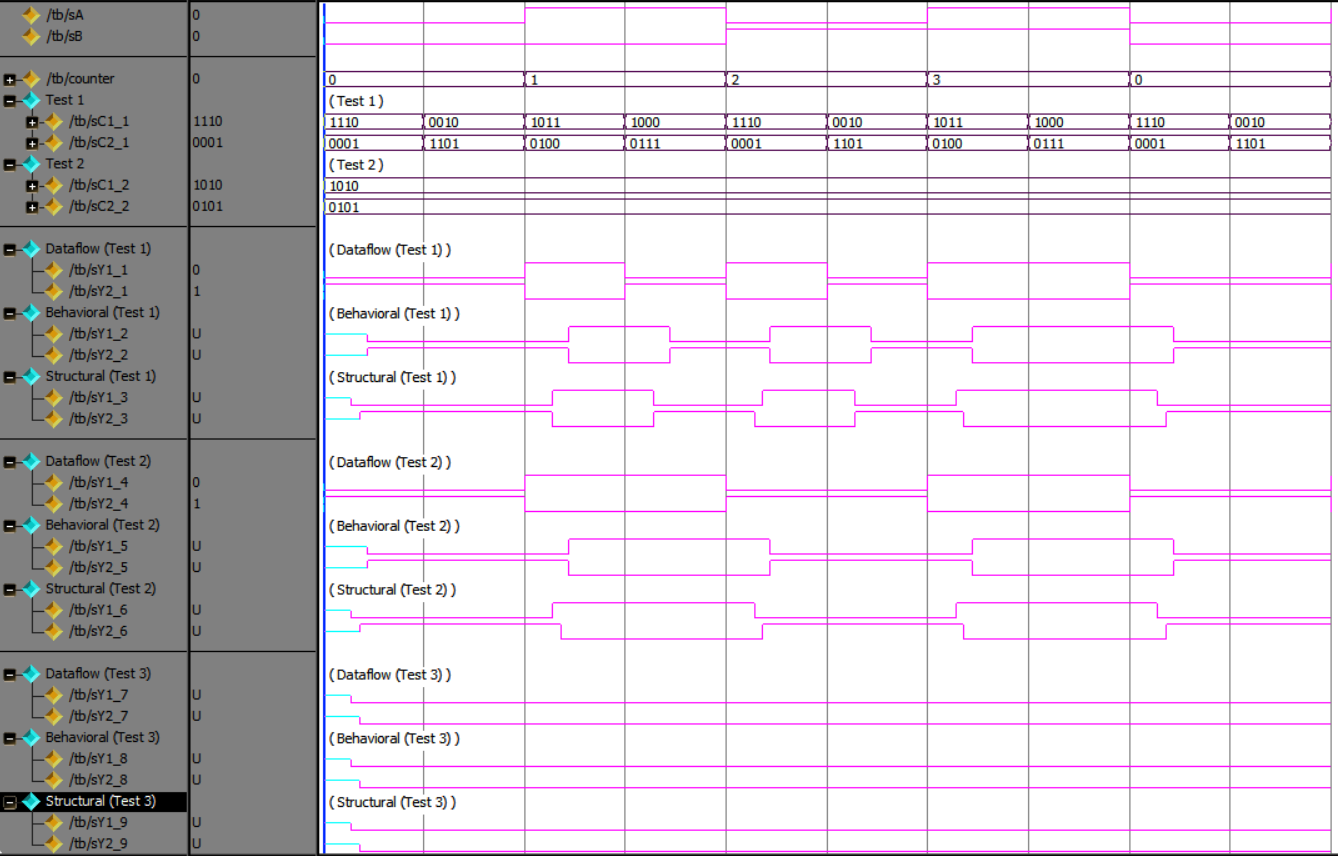
\includegraphics[width=\textwidth]{capture}
	\caption{Wave captures I/O of all three tests.}
	\label{fig:capture}
\end{figure}

The wave output yielded expected results. Inputs for test set 1, \texttt{C1\_1} and \texttt{C1\_2}, left shifted every $50\,\si{\nano\s}$ as well as swapped places. The BA counter used for all Three test sets was incremented every $100\,\si{\nano\s}$. Test set two has a constant set of inputs into each mux. Test set three has a HIGH input into both of its strobes and therefore yields a LOW signal during the entire test.

\section*{Conclusion}

In this laboratory exercise, the functionality of a 74LS153 chip was emulated in three ways in VHDL. A dataflow implementation with no propagation delay, a behavioral with worst case delay, and a structural with individual delays for each gate were created. Three test sets with varying inputs were created to succinctly test the circuit. A wave capture was recorded to verify the integrity of the circuit. The exercise was successful as the desired outputs were attained from the original circuit and the test bench verified this integrity.

\section*{Questions}

A circuit with inputs, a b c d, internal signals, u v w x y, and output z was defined.

\begin{figure}[h!]
	\centering
	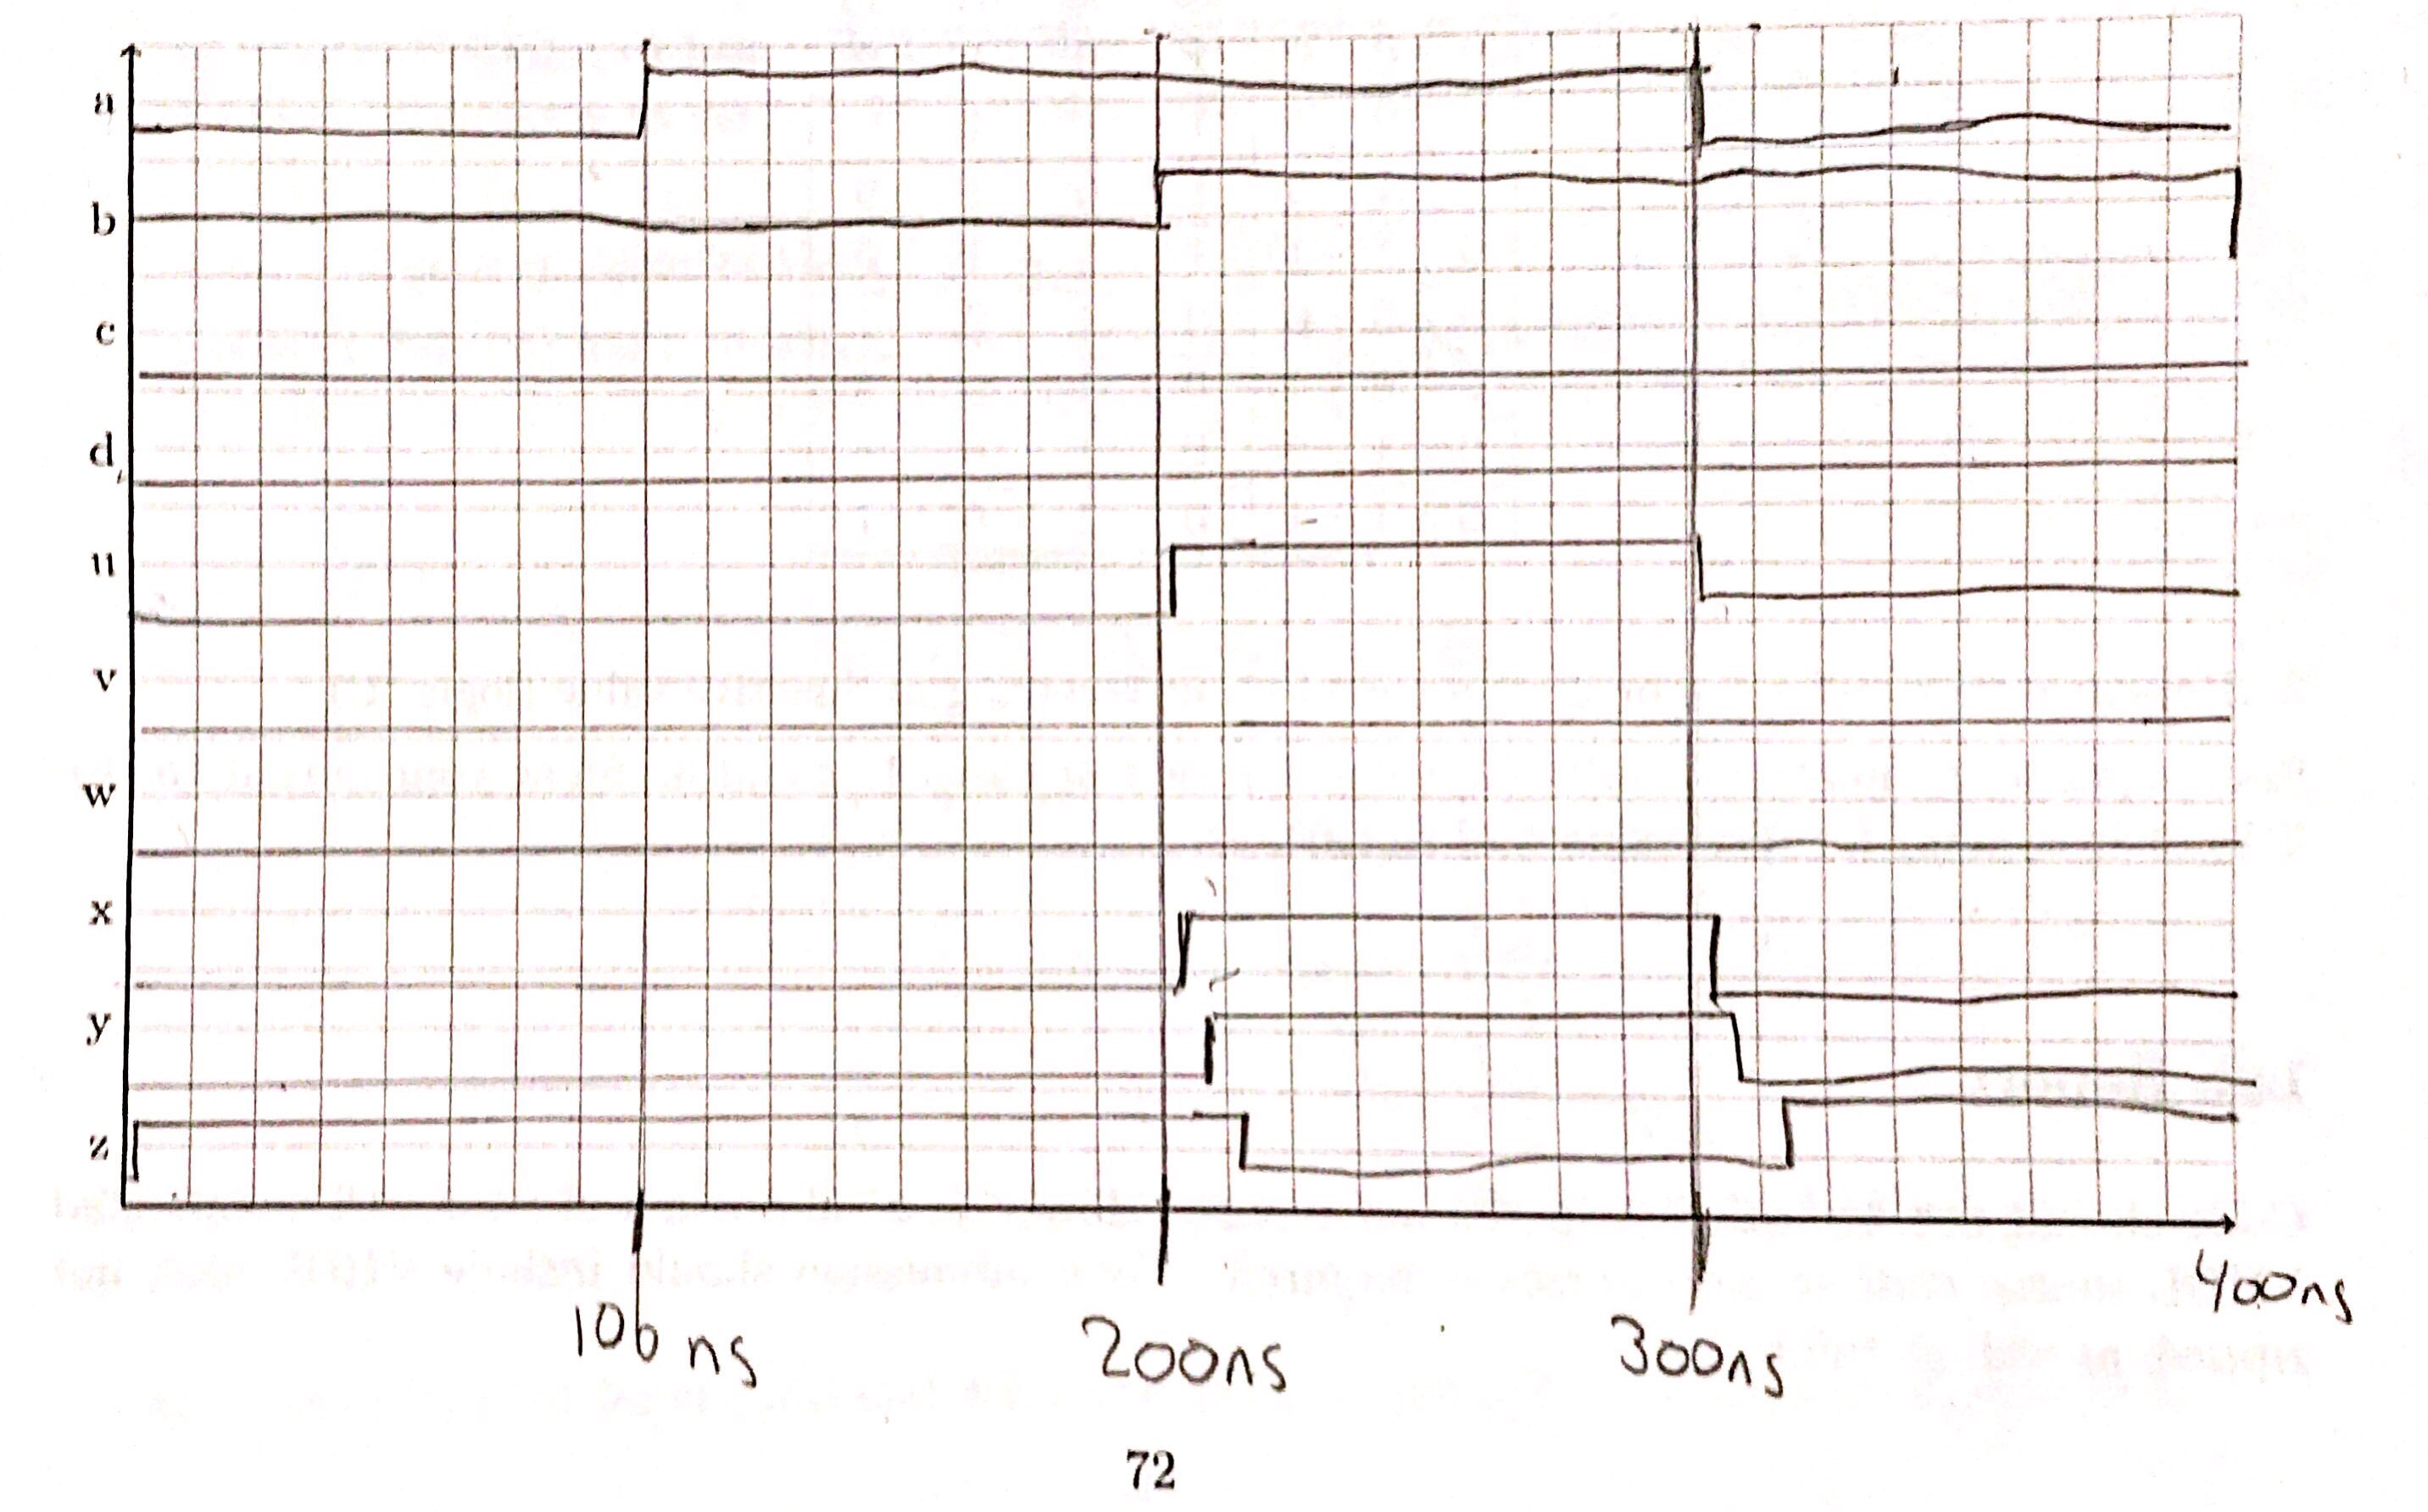
\includegraphics[width=\textwidth]{question}
	\caption{Wave capture of the defined circuit.}
	\label{fig:capture-q1}
\end{figure}

Figure \ref{fig:capture-q1} shows a wave capture generated over a $400\,\si{\nano\s}$ period.
\pagebreak
\begin{figure}[h!]
	\centering
	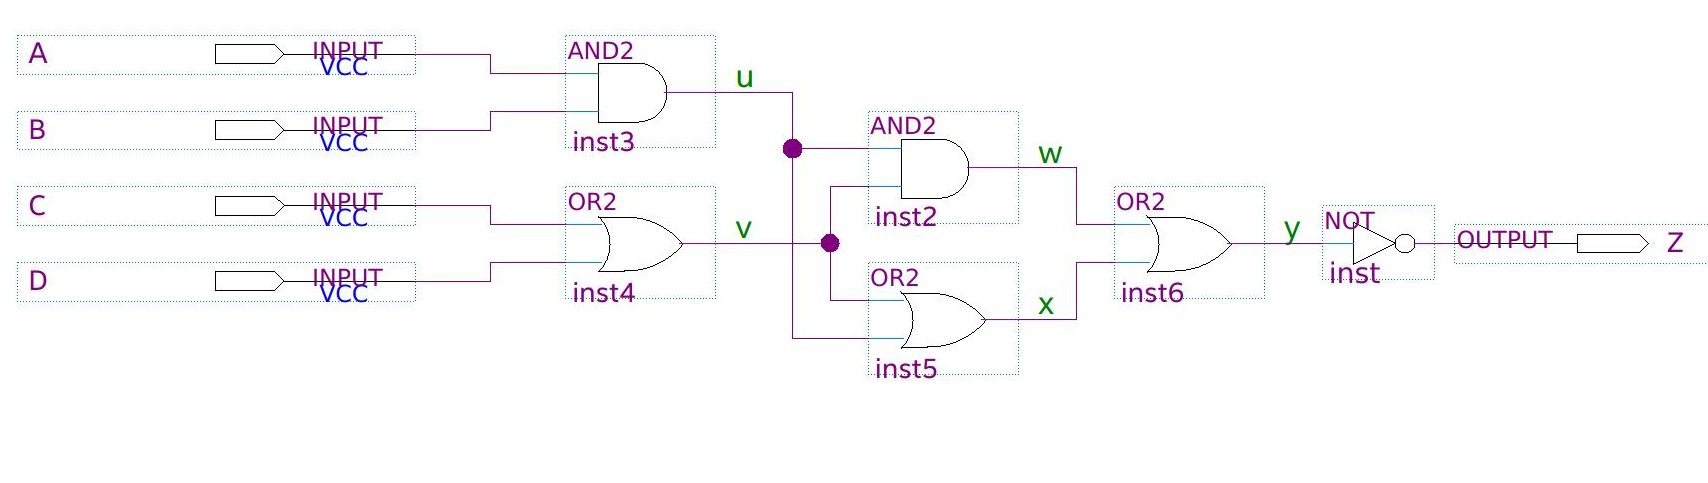
\includegraphics[width=\textwidth]{question_schem}
	\caption{Wave capture of the defined circuit.}
	\label{fig:q1-schem}
\end{figure}

The circuit was drawn in Quartus and the internal and external signals were labeled in Figure \ref{fig:q1-schem}.

\end{document}
